\documentclass[12pt]{article}
%使用xeCJK宏包来支持中英文混排,控制序列设置CJK主字体
\usepackage{xeCJK}
\setCJKmainfont{Adobe Song Std}

%编辑数学公式
\usepackage{amsmath}

%控制首行缩进,latex默认不缩进,并设置首行缩进两个字符位置
\usepackage{indentfirst}
\setlength{\parindent}{2em}

%在LaTex中插入图片的宏包
\usepackage{graphicx}

\title{Latex 使用实例}
\author{nobody}
\date{\today}
\begin{document}
\maketitle
\section{你好中国}
中国在East Asia.
\subsection{Hello Beijing}
北京是capital of china
\subsection{Hello Dongcheng District}
\paragraph{Tian'anmen Square}
is in the center of Beijing
\subparagraph{Chairmen Mao}
is in the center of 天安门广场
\subsection{Hello 山东}
\paragraph{山东大学}is one of the best university in 山东

\section{数学公式}
\subsection{行内公式和行间公式}
Einstein's $E=mc^2$.
%上标和下标表示
\begin{equation}
Z = R \cdot e^{2 \pi i}.
\end{equation} 
$X = x_1 + x_2$.

\subsection{根式与分式}
$\sqrt{e^3}$\\[5pt]
$\sqrt[3]{x^{2 \pi t}}$\\[5pt]
$\frac{1}{x_2}$
\begin{equation}
Z = \frac{1}{x_1}.
\end{equation}
$\dfrac{1}{x_3}$\\[5pt]

\subsection{运算符}
\subsubsection{连加}
$ \sum_{i=1}^n i $
\subsubsection{连乘}
$ \prod_{i=1}^n i $
\subsubsection{不压缩上下标的连加乘}
%\quad表示空格
$ \sum\limits _{i=1}^n i\quad \prod\limits _{i=1}^n i $
\subsubsection{极限和积分}
$ \lim_{x\to0}x^2 \quad \int_a^b x^2 dx $
\subsubsection{压缩上下标的极限和积分}
$ \lim\nolimits _{x \to 0}x^2 \quad \int\nolimits_a^b x^2 dx $
\subsubsection{多重积分}
$ \iint \quad \iiint \quad \iiiint \quad \idotsint $
\subsubsection{定界符}
\[
\Biggl(\biggl(\Bigl(\bigl((x)       \bigr)\Bigr)\biggr)\Biggr)
\]

\[
\Biggl[\biggl[\Bigl[\bigl[[x]\bigr]\Bigr]\biggr]\Biggr]
\]

\[
\Biggl \{\biggl \{\Bigl \{\bigl \{\{x\}\bigr \}\Bigr \}\biggr \}\Biggr\}
\]

\[
\Biggl\langle\biggl\langle\Bigl\langle\bigl\langle\langle x
\rangle\bigr\rangle\Bigr\rangle\biggr\rangle\Biggr\rangle 
\]

\[ 
\Biggl\lvert\biggl\lvert\Bigl\lvert\bigl\lvert\lvert x
\rvert\bigr\rvert\Bigr\rvert\biggr\rvert\Biggr\rvert 
\]

\[ 
\Biggl\lVert\biggl\lVert\Bigl\lVert\bigl\lVert\lVert x
\rVert\bigr\rVert\Bigr\rVert\biggr\rVert\Biggr\rVert 
\]
\subsubsection{省略号}
\[
 x_1,x_2,\dots ,x_n
 \quad 
 1,2,\cdots ,n
 \quad
 \vdots
 \quad 
 \ddots 
\]
\subsubsection{矩阵运算符}
\[ 
\begin{pmatrix} 
	a&b\\c&d 
\end{pmatrix} \quad
\begin{bmatrix} 
	a&b\\c&d \end{bmatrix} \quad
\begin{Bmatrix} 
	a&b\\c&d \end{Bmatrix} \quad
\begin{vmatrix} 
	a&b\\c&d \end{vmatrix} \quad
\begin{Vmatrix} 
	a&b\\c&d \end{Vmatrix} 
\]

%生成行内公式的小矩阵
Marry has a little matrix $ ( \begin{smallmatrix} a&b\\c&d \end{smallmatrix} ) $.

\subsection{多行公式}
%无需对齐的长公式可以使用multline环境
\begin{multline*}
x = a+b+c+{}\\
d+e+f+g
\end{multline*}

%需要对齐的长公式,可以使用aligned次环境来实现,它必须包含在数学环境之内
\[
\begin{aligned}
x={}&a+b+c+{}\\
&d+e+f+g
\end{aligned}
\]

%无需对齐的公式组可以使用gather环境,需要对齐的公式组可以使用align环境。加上*可以去除编号
\begin{gather}
a=b+c+d\\
x=y+z
\end{gather}
\begin{align}
a &= b+c+d\\
x &= y+z
\end{align}

\subsection{分段函数}
%分段函数可以用cases次环境来实现,它必须包含在数学环境之内。
\[
y=\begin{cases}
-x, \quad x\leq 0\\
x, \quad x>0
\end{cases}
\]

\section{插入图片和表格}
\subsection{插入图片}
\begin{figure}[htbp]
\centering
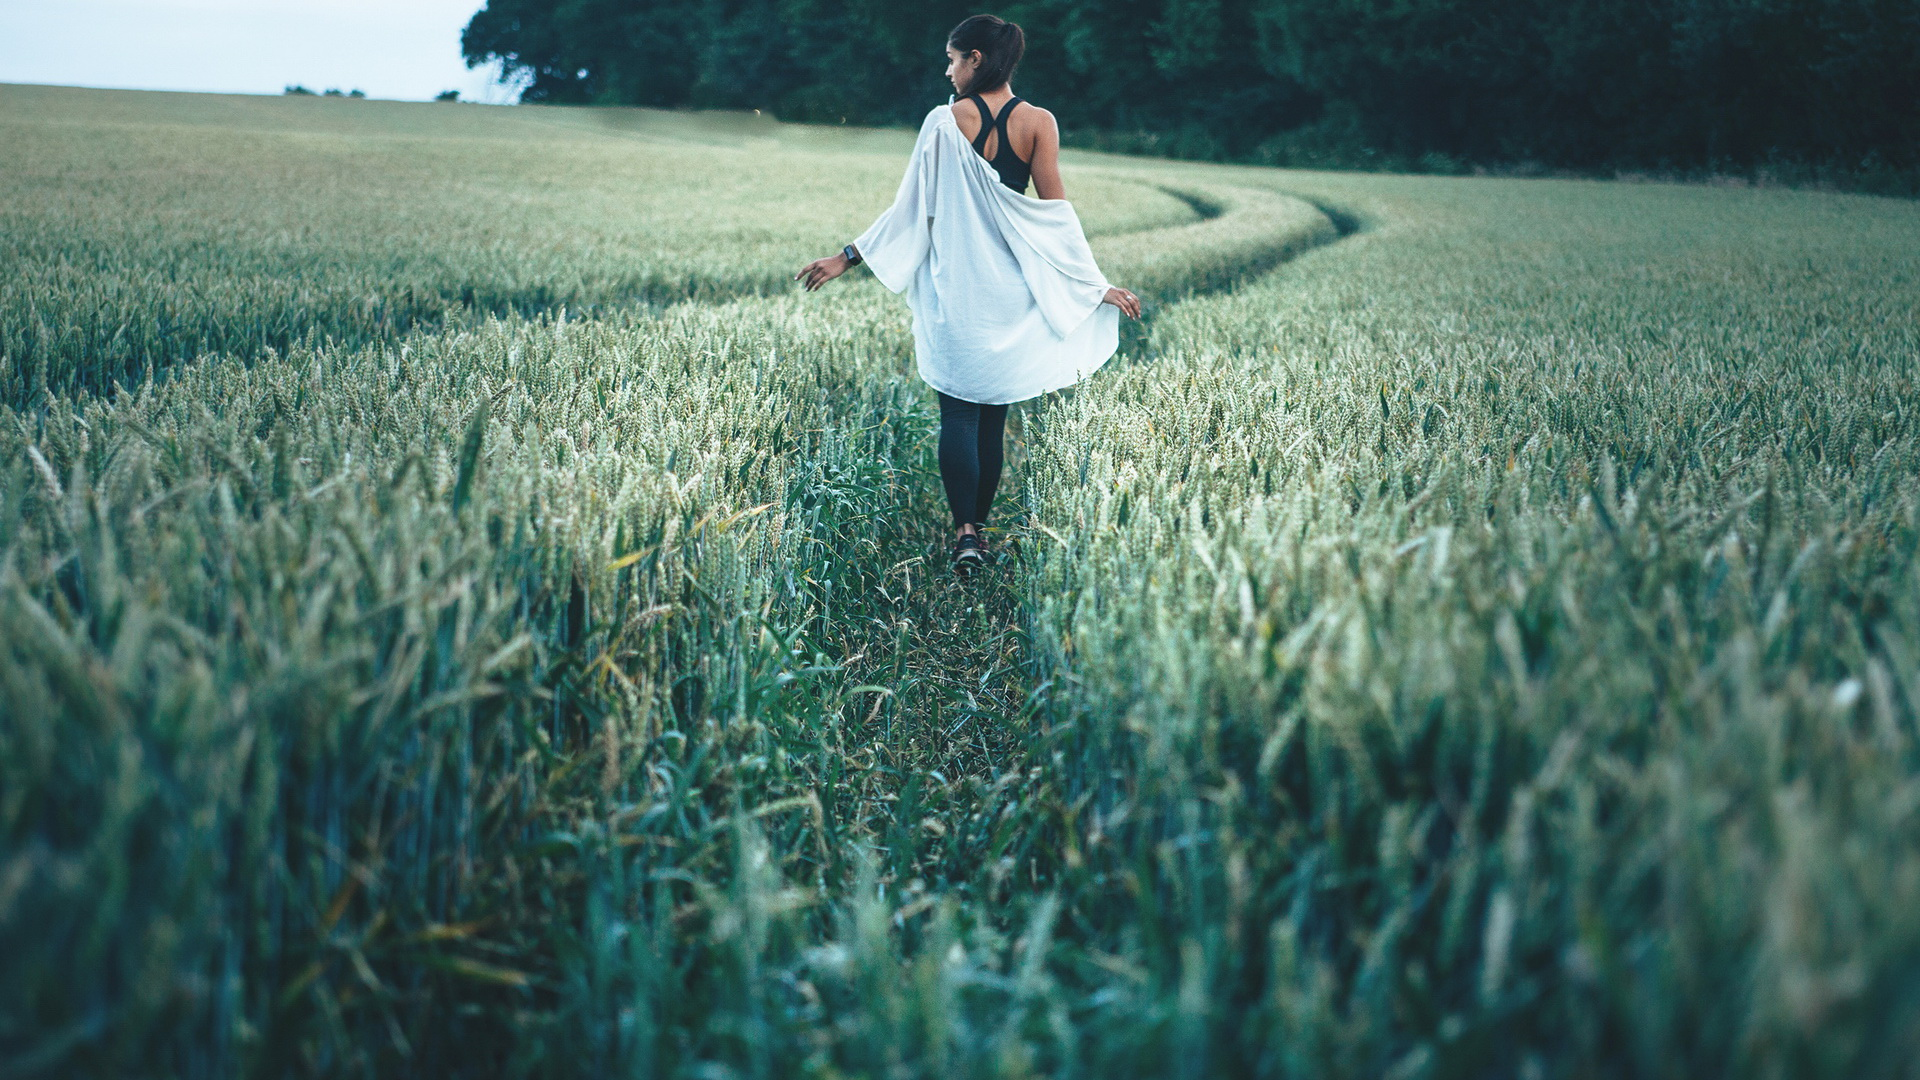
\includegraphics[angle=-30,totalheight=20mm,
width=30mm,keepaspectratio]{a.jpg}
\caption{有图有真相}
\label{fig:myphoto}
\end{figure}

\subsection{插入表格}
%tabular环境提供了最简单的表格功能
%\hline 表示横线,在列表格中用|表示竖线,&来分列,\\来换行
%每列可以采用居左、居中、居右等横向对齐方式,通过使用l, c, r来表示
\begin{tabular}{|l|c|r|}
 \hline
操作系统& 发行版& 编辑器\\
 \hline
Windows & MikTeX & TexMakerX \\
 \hline
Unix/Linux & teTeX & Kile \\
 \hline
Mac OS & MacTeX & TeXShop \\
 \hline
通用& TeX Live & TeXworks \\
 \hline
\end{tabular}

\end{document}